\documentclass[a4paper]{article}

% Language and font encodings
\usepackage[english]{babel}
\usepackage[utf8x]{inputenc}
\usepackage[T1]{fontenc}
\usepackage[a4paper,top=3cm,bottom=2cm,left=3cm,right=3cm,marginparwidth=1.75cm]{geometry}
\usepackage{amsmath}
\usepackage{titlesec}
\usepackage{graphicx}
\usepackage{tabularx}
\usepackage{natbib}
\usepackage[colorinlistoftodos]{todonotes}
\usepackage[colorlinks=true, allcolors=blue]{hyperref}
\usepackage{caption}
\usepackage{subcaption}
\usepackage{multicol}
\setlength{\columnsep}{1cm}
\usepackage{listings}
\usepackage{parskip} 			%turns off automatic indentation
\usepackage{setspace}
\usepackage{hyperref}
\hypersetup{
    colorlinks=true,
    linkcolor=blue,
    filecolor=magenta,      
    urlcolor=cyan,
}
\urlstyle{same}
\begin{document}

	\begin{center}
	  {\huge FYS4150 - Project 4}\\[2ex]
      {\huge Crafting and Investigating the Ising Model}\\[8ex]
	  {\large Daniel Herman}\\[4ex]
      \normalsize
      \today
	\end{center}

\begin{abstract}
The Ising model is a commonly utilized model of statistical systems. In this project, we create our own Ising model using the programming language c++. The code is parallelized using OpenMPI, and python programs were written to extract and plot data output by the c++ program. The Monte Carlo Markov Chain is used to cycle through our model, and accepted changes to the model are determined using the Metropolis algorithm. Both of these methods utilize random number generators picking from a uniform distribution. This approach has proved very successful for run times of at least $10^6$ Monte Carlo cycles, showing convergence to the analytical solutions predicted by statistical mechanics.
\end{abstract}
\clearpage

\section{Introduction}\label{intro}
The Ising Model is a common way to analyze phase transitions for physical phenomena. In this project, we look at the two-dimensional Ising Model. For this specific case, we're looking at the phase transition between a magnetized state, and a state with no magnetization. Each lattice site is binary, in that it can take one of two possible states, namely spin up, or spin down. In the initial state, all of the lattice site spins are either aligned, giving a fully magnetized system, or randomly distributed. As the temperature of the system changes, the spin orientation of each lattice site has a potential to change as determined by the Boltzmann distribution described in section \ref{methods}. The total energy of the lattice at any given moment is given by the simple relation
\begin{equation}\label{eq:mesh1}
E=-J\sum_{< kl >}^{N}s_ks_l 
\end{equation}
where $s_k = \pm 1$. $N$ represents the total number of spins and $J$ is a coupling constant that expresses the strength of the interaction between neightboring spins. For ease, we scale our calculations by setting $J=1$. The lower index of the sum $<kl>$ states that we only sum over the nearest neighbors.\\
We investigate the two-dimensional case of the Ising model specifically as it has analytical expressions for the expectation values of the quantities which we study through our simulation. We can utilize these analytical expressions to compare with our results in section \ref{results}.

\section{Methods}\label{methods}
In order to understand the results of our Ising model simulation, we have to investigate the analytical expressions of the Ising model as well as Monte Carlo cycles and the Metropolis algorithm.
\subsection{The Ising Model}\label{ising}
We use analytic expressions of the Ising model to help understand the behavior of the model, and verify the results of our code. We find analytic expressions for the energy expectation value $<E>$, the mean absolute value of the magnetic moment (mean magnetizaion) $<|M|>$, the specific heat $C_V$ and the susceptibility $\chi$ as functions of the temperature $T$. In order to find these expressions, we first must clarify some information about the Ising model.\\

\subsection{Probability Distribution Function (PDF).}
The energy of the system is described in equation \ref{eq:mesh1}. The probability of finding an energy $E_i$ at a given temperature $T$ is given by the Boltzmann distribution
\begin{equation}
P_i(T) \propto e^{-E_i/k_BT}
\end{equation}
For simplification, we redefine the quantity $\dfrac{1}{k_BT} = \beta$, and scale the distribution by setting $k_B=1$. In order to find the actual probability value for each energy, we introduce a normalization constant
\begin{equation}\label{eq:boltz}
P_i(\beta) = \dfrac{e^{-E_i\beta}}{Z}
\end{equation}
where $Z = \sum_{i=1}^Me^{-E_i\beta}$ is the partition function of the distribution. $M$ is the number of possible spin configurations.\\

\subsection{Analytical Expectation Values.}
Now we can calculate the expectaion value for the energy in the typical fashion
\begin{equation}\label{eq:expece}
<E> = \sum_{i=1}^ME_iP_i(\beta)
\end{equation} 
We utilize the PDF again to determine the mean magnetization as well, using the definition of the magnetization of a state $M_i = \sum_{i=1}^ds_i$ where $s_i = \pm 1$ is the value of spin $i$.
\begin{equation}\label{eq:expecm}
<|M|> = \sum_{i=1}^MM_iP_i(\beta)
\end{equation}
Similarly, we calculate the values $<E^2>$ and $<M^2>$ so that we can determine the variance $\sigma^2$ of the energy and magnetization values.
\begin{align*}
<E^2> =& \sum_{i=1}^ME_i^2P_i(\beta)\\
<M^2> =& \sum_{i=1}^MM_i^2P_i(\beta)\\
\sigma_E^2 =& <E^2>-<E>^2\\
\sigma_M^2 =& <M^2>-<M>^2
\end{align*}

\subsection{Analytical Specific Heat and Susceptibility.}
Using some statistical mechanics tricks, we can drive the specific heat $C_V$ and magnetic susceptibility $\chi$ expressions given below
\begin{align}
C_V =& \dfrac{\sigma_E^2}{k_BT^2}\\
\chi =& \dfrac{\sigma_M^2}{k_BT} 
\end{align}

\subsection{Computational Energy Expectation Value.}
However, as the number of spins increases, calculating the partition function becomes more and more taxing. So in our case, instead of attempting to calculate the partition function, we average the energies found after each Monte Carlo (MC) cycle by dividing by the number of MC cycles $N$ as such. 
\begin{align}
<E> \simeq \dfrac{1}{N}\sum_{i=1}^N E_i, & <M> \simeq \dfrac{1}{N}\sum_{i=1}^N M_i\\
<E^2> \simeq \dfrac{1}{N}\sum_{i=1}^N E_i^2, & <M^2> \simeq \dfrac{1}{N}\sum_{i=1}^N M_i^2
\end{align}

\clearpage

\subsection{Phase Transitions.}\label{phasetrans}

When the system approaches a phase transition, the physical quantities expressed above evolve as a function of the temperature difference between the systems temperature $T$, and the critical temperature $T_C$. These relations are found in \cite{Project4Guide}. Important quantities change as follows

\begin{align}\label{relations}
<M(T)> \sim& (T-T_C)^{\beta}\\
C_V(T) \sim& |T_C-T|^{\alpha}\\
\chi(T) \sim& |T_C-T|^{\gamma}
\end{align}
Where the experimental values are $\beta = 1/8$, $\alpha = 0$, and $\gamma = 7/4.$

For our model the functionality of the above relations is dependent upon the correlation length, which charaterizes the strength correlation between different part of the lattice. When the temperature approaches $T_C$, the spins become more correlated with one another and the correlation length should span the entire lattice. The behavior of $\zeta$ near $T_C$ is

\begin{equation}\label{eq:corr}
\zeta(T) \sim |T_C-T|^{-\nu}
\end{equation}

As a result of this change in correlation length, we can relate the behavior of finite lattices to the results from an infinitely large lattice. We see that the critical temperature scales according to the size of the lattice $L$ by
\begin{align*}
T_C(L) - T_C(L=\infty) = aL^{-1/\nu}
\end{align*}

Substituting this back into \ref{relations}, where we set $T=T_C$,

\begin{align*}
<M(T)> \sim (T-T_C)^{\beta} \rightarrow L^{-\beta/\nu} \\
C_V(T) \sim |T_C-T|^{-\alpha} \rightarrow L^{\alpha/\nu}\\
\chi(T) \sim |T_C-T|^{-\gamma} \rightarrow L^{\gamma/\nu}
\end{align*}

\subsection{Monte Carlo Cycles}
The Monte Carlo method is a very popular way to solve complex probabilistic problems not only in physics but in other fields such as economics. It is often used when the changes of the system simulated are not deterministic in nature. Monte Carlo methods use randomly selected variables from a probability distribution to make changes in the system. This is particularly useful in the Ising model simulation as the behavior over time is statistical in nature.
\subsection{Metropolis Algorithm}
The Metropolis algorithm was crafted to estimate distribution functions (PDF1) by making random samples based off of a different distribution (PDF2) which is proportional to the distribution function we want to find. For each iteration of the algorithm, the random sample is not always accepted. The move is accepted or denied based off of PDF1. If the random move selected moves towards a position with higher probability then it is accepted. This will quickly cause the distribution of random samples to look like PDF1.
\clearpage
\subsection{Code Parallelization}
The code we run is not very memory intensive, however it makes many many calculations per second, especially as the lattice size increases. Because our analysis is statistical in nature, and our code is random in nature, we want to look at many iterations of our code for different lattice sizes. We want to run each lattice with $10^6$ MC cycles many times to be able to study the behavior of our model. In order to save time with our calculations, we will use many processors simultaneously. We utilize OpenMPI, which is an open source Message Passing Interface to parallelize our code. Our code is simple to parallelize, because the processors do not need to communicate with each other while the code is running. Each processor can run the code independently. The output files are sent to the master compter for analysis. 
\clearpage


\section{Implementation}\label{implementation}
Code is written in c++ to create the Ising model and can be found at \url{https://github.com/hermda02/Project4}. The Monte Carlo method and the Metropolis algorithm are applied in the code. I will describe the behavior of these methods for our specific case below.
\subsection{Monte Carlo Cycles}
For our model to behave in a realistic matter, we cannot expect the flipping of spins to be deterministic. We implement the Monte Carlo Markov Chain to simulate a random flipping of spins.  In order to do that, we create a loop over all the spins in the lattice, picking one randomly using a randomizer picking from a normal distribution. Since we have a two dimensional lattice, first we pick a random row, then a random column. We determine whether or not the spin is flipped based off of the Metropolis algorithm. For each Monte Carlo cycle, we randomly pick $N$ spins, one by one, where $N$ is the total number of spins in the lattice. This means that the same spin could potentially be flipped multiple times, and some spins may never be selected during the course of a Monte Carlo cycle.
\subsection{Metropolis Algorithm}
Once a spin has been selected, the current energy of that spin $E$ is calculated. If the spin were to be flipped, the change in energy of the system would be equal to $2*E$ (i.e. if the spin has an energy $E=4$, when it is flipped, the energy becomes $E=-4$, so the change in energy $|\Delta	E| = 8$). This value $\Delta E$ is then used to calculate the probability of the spin changing, according to the Boltzmann distribution \ref{eq:boltz}. The use of the Boltzmann distribution is handy, as the maximum value $P_i$ can take is when $\Delta E=0$, where $P_i = 1$. A random number, $x$ is then picked from a normal distribution ($x \in [0,1]$), and if $x \leq P_i$, then the spin is flipped. This guarantees that as the model evolves, the lattice moves towards the most probabilistic state.
\subsection{Parallelization and Optimization}
We utilize OpenMPI in our c++ code. At the Institute for Theoretical Astrophysics (ITA), we have access to many super computer clusters. We use our access to the beehive cluster to run our code quickly and efficiently. This is optimal for producing large data sets necessary for in depth analysis of our model. More information on ITA's computing resources can be found at: \url{http://www.mn.uio.no/astro/english/services/it/help/basic-services/compute-resources.html}.
\clearpage

\section{Results}\label{results}
To understand the behavior of our Ising model, we investigate lattices of different sizes $L$ and at different temperatures $T$. All lattices that we investigate are square ($L$ x $L$). To verify that our code behaves as we would like, we compare the results from the $L=2, T=1$ case to the analytical expressions for this case. According to our analytical expressions, if the code is working as expected we would see $<E> = -2$ (minimized energy), and we would expect the system to remain in and ordered magnetic state $<|M|>=1$. According to our results, our code is behaving as expected, with an ordered final state $<|M|> = 1$ and minimized energy $<E> = -2$. The number of Monte Carlo cycles it takes for our code to reach a steady state is very small ($<10^3$) in this case, which is expected as there are only 4 potential spin flips per MC cycle. The analytical expressions becomes very difficult to calculate as the size of the lattice increases, so future analysis will focus more on comparing trends rather than specific values.

\subsection{Number of MC Cycles until Convergence}

To better understand the number of MC cycles it takes for the lattice to reach a steady state, we look at a larger case. We set $L=20$, and look at the $T=1$ and $T=2.4$ case. The evolution of $<E>$ as a function of MC cycles is shown below.

\begin{figure}[ht!]
\centering
\begin{minipage}[t]{0.45\textwidth}
\centering
\includegraphics[scale=0.4]{partc/T1.0/ordered/Eexpec}
\captionof{figure}{$<E>$ as a function of MC cycles for $T=1.0$, with an ordered initial state.}
\label{fig:mesh1}
\end{minipage}
\begin{minipage}[t]{0.45\textwidth}
\centering
\includegraphics[scale=0.4]{partc/T1.0/random/Eexpec}
\captionof{figure}{$<E>$ as a function of MC cycles for $T=1.0$, with an random initial state.}
\label{fig:mesh2}
\end{minipage}
\end{figure}

\begin{figure}[ht!]
\centering
\begin{minipage}[t]{0.45\textwidth}
\centering
\includegraphics[scale=0.4]{partc/T2.4/ordered/Eexpecs}
\captionof{figure}{$<E>$ as a function of MC cycles for $T=2.4$, with an ordered initial state.}
\label{fig:mesh3}
\end{minipage}
\begin{minipage}[t]{0.45\textwidth}
\centering
\includegraphics[scale=0.375]{partc/T2.4/random/Eexpec}
\captionof{figure}{$<E>$ as a function of MC cycles for $T=2.4$, with an random initial state.}
\label{fig:mesh4}
\end{minipage}
\end{figure}

As seen in figures \ref{fig:mesh1}, \ref{fig:mesh2}, \ref{fig:mesh3} and \ref{fig:mesh4}, it takes between $10^5$ and $10^6$ MC cycles to reach an equilibrium state. Knowing this, we will use $10^6$ MC cycles for the remainder of our calculations, to ensure that our simulations reach a steady state. The figures above only show the energy, yet the same converging  behavior is observed for the other physical quantities.\\

For each MC cycle, there are $N^2$ opportunities for a spin to flip (where $L=N$.) The spin is only flipped if the new configuration of the lattice is accepted according to the Boltzmann distribution. Below is a plot of the log-log plot of the number of accepted configurations as a function of MC cycles. The number of accepted states grows linearly with MC cycles. Comparing figures \ref{fig:mesh10} and \ref{fig:mesh24} shows us that there are more accepted configurations for higher $T$.

\begin{figure}[ht!]
\centering
\begin{minipage}[t]{0.45\textwidth}
\centering
\includegraphics[scale=0.4]{partc/T1.0/random/acceptconfigs}
\captionof{figure}{Number of accepted states as a function of MC cycles for $T=1.0$, with a random initial state.}
\label{fig:mesh10}
\end{minipage}
\begin{minipage}[t]{0.45\textwidth}
\centering
\includegraphics[scale=0.4]{partc/T2.4/random/acceptconfigs}
\captionof{figure}{Number of accepted states as a function of MC cycles for $T=2.4$, with a random initial state.}
\label{fig:mesh24}
\end{minipage}
\end{figure}

 

\clearpage
\subsection{Lattice Behavior}

Now that we know how much time it takes before the lattice converges to values, we can study the lattice after convergence to truly see how our model behaves for different sizes and temperatures.

\subsubsection{Energy Probability}
Once the system has reached a steady state, there is still a possibility that spins flip, and the total energy of the system "floats" around the steady state value. We store the values of the energy after the system becomes stable, making a histogram of the potential values of the energy of the system. The energy of the system is stored after each MC cycle, for $10^5$ MC cycles after the lattice has reached an equilibrium state ($10^6$). 

\begin{figure}[ht!]
\centering
\begin{minipage}[t]{0.45\textwidth}
\centering
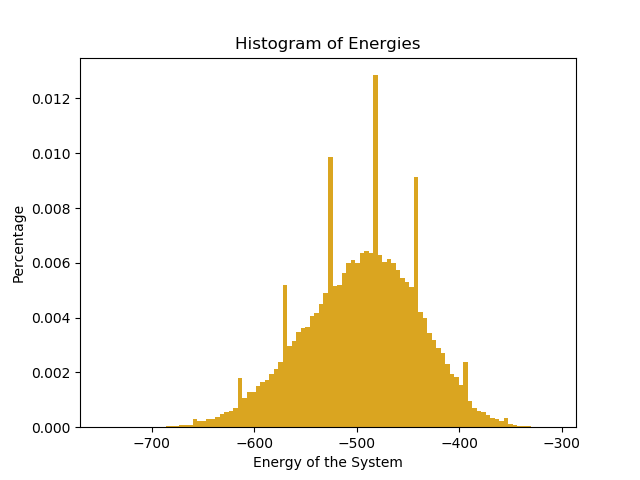
\includegraphics[scale=0.4]{partd/T2.4/after10+6histo}
\captionof{figure}{Energy distribution of $10^5$ MC\\ cycles after reaching equilibrium, for\\ $T=2.4$.}
\label{fig:energydist1}
\end{minipage}
\begin{minipage}[t]{0.45\textwidth}
\centering
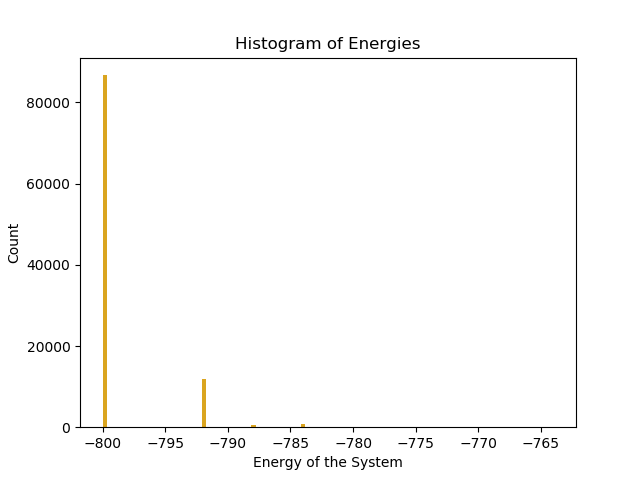
\includegraphics[scale=0.4]{partd/T1.0/energyhisto}
\captionof{figure}{Energy distribution of $10^5$ MC cycles after reaching equilibrium, for\\ $T=1.0$.}
\label{energydist2}
\end{minipage}
\end{figure}

The probability distribution at $T=2.4$, figure \ref{fig:energydist1} follows the Boltzmann distribution well, however we notice large spikes at the stable, most likely states at the given temperature. Even the most likely state has a probability on the order of $1\%$.

When $T=1.0$ the system is sitting in an ordered state, with minimized energy as seen in figure \ref{energydist2}. As a result, the probability of the lattice remaining in this minimized state, $E = -800$, is dominant (86.7$\%$), and the next most common state, $E = -792$ (11.9$\%$). Every other populated state ($E = -788, -784,-780,-776$) all have probabilities of under $1\%$.

\clearpage

\subsubsection{Phase Transitions}\label{phaser}
Comparing the behavior of our model at $T=1.0$ and $T=2.4$, we can see that there is some sort of transition in this temperature range. We investigate further, and find that there is a distinct change within the temperature range of $T \in [2.1,2.4]$. We run our simulation for this range of temperatures, with temperature steps of 0.02. Different sized lattices are used as well.

\begin{figure}[ht!]
\centering
\begin{minipage}[t]{0.45\textwidth}
\centering
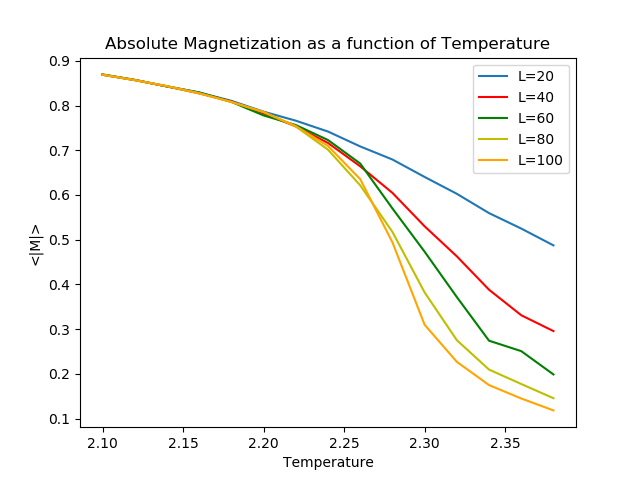
\includegraphics[scale=0.4]{parte/AbsMagnet}
\captionof{figure}{$<|M|>$ as a function of temperature.}
\end{minipage}
\begin{minipage}[t]{0.45\textwidth}
\centering
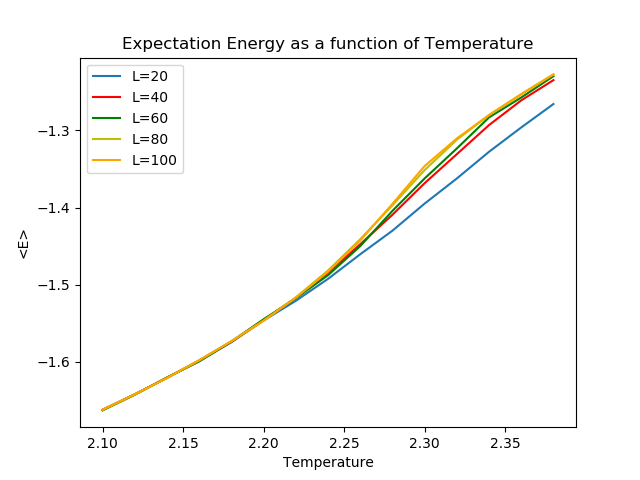
\includegraphics[scale=0.4]{parte/EnergyExpec}
\captionof{figure}{$<E>$ as a function of temperature.}
\end{minipage}
\end{figure}

The trends of the expectation values of the energy and absolute value of magnetization look more functional as the lattice size increases, following the relations as show in \ref{phasetrans}. Something is causing a slight change in system energy, but a large change in magnetization in the range $T \in [2.25 - 2.30]$.

\begin{figure}[ht!]
\centering
\begin{minipage}[t]{0.45\textwidth}
\centering
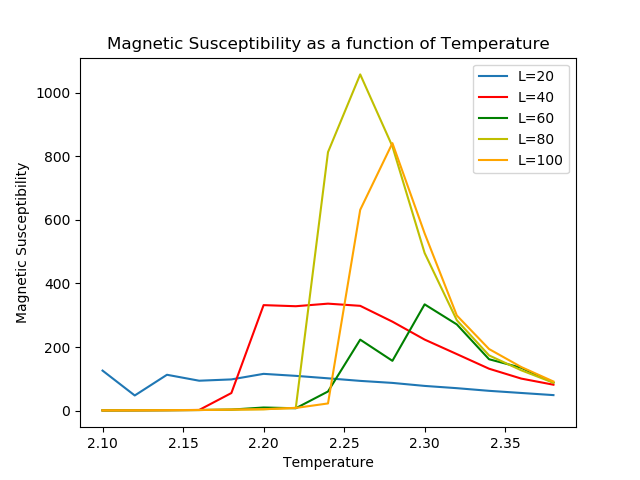
\includegraphics[scale=0.4]{parte/MagnetSus}
\captionof{figure}{$\chi$ as a function of temperature.}
\label{fig:meshsus}
\end{minipage}
\begin{minipage}[t]{0.45\textwidth}
\centering
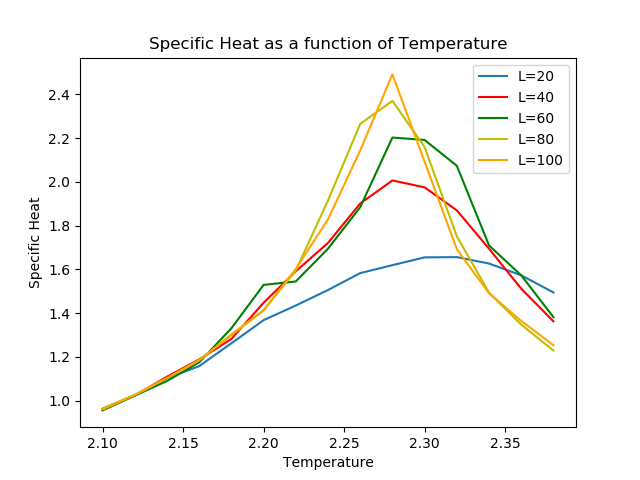
\includegraphics[scale=0.4]{parte/SpecificHeat}
\captionof{figure}{$C_V$ as a function of temperature.}
\label{fig:meshspecheat}
\end{minipage}
\end{figure}

When we plot the behavior of the magnetic susceptibility $\chi$ (fig. \ref{fig:meshsus}) and the specific heat $C_V$ (fig. \ref{fig:meshspecheat}), we see that there is a drastic change in the range $T \in [2.25 - 2.30]$. We also see that the stability and resolution of these changes become more defined as the lattice size increases. 

To find a more where this critical temperature $T_C$ is located, we need to make some approximations using the relations used in in \ref{phasetrans}. First, we want to solve for the correlation length proportionality constant $a$. We are utilizing equations (12) and (13) and magnetic susceptibilty values from our data at apparent peaks, assuming the peaks are near the critical temperature. We use the given values for $\gamma = 7/4$ and $\nu = 1$.

\begin{align*}
\chi_i(T) = 1057.17 \sim aL^{\gamma/\nu} = a80^{7/4}\\
\chi_f(T) = 841.134 \sim aL^{\gamma/\nu} = a100^{7/4}\\
a \simeq \dfrac{1057.17-841.134}{80^{7/4}-100^{7/4}} = -0.2113
\end{align*}

\clearpage

Using equation \ref{eq:corr}, and the accepted value given ($T = 2.269$)

\begin{align*}
T_C(L) - T_C(L = \infty) = aL^{1/\nu}\\
T_C(100) - 2.269 = (-0.2113)*100^{-1}\\
T_C(100) = 2.269 - 2.113*10^{-3} = 2.2668
\end{align*}

For a 100x100 lattice, we find a critical temperature with a relative error of 0.001 from the accepted value. 

\clearpage

\section{Discussion}\label{discussion}

The code for this project was simple to create, and utilizes helpful c++ libraries such as armadillo and random. It runs quickly for small lattice sizes, but as the size of our simulation grows, the computation time grows accordingly. OpenMPI cut down significantly on the time, especially with access to the supercomputers at ITA. On standard laptops, the code for the larger simulations used in this project take on the order of 10s of hours, but with the super computers at ITA, the computations take on the order of 10s of minutes.

The Monte Carlo Markov Chain and the Metropolis algorithm have proven very successful in solving this problem. Both of these methods involve random moves, and the Metropolis algorithm utilizes calculated probabilities inherent to the problem. As a result, for "small" number of MC cycles, the results appear random with slow convergence. However, after roughly $5*10^5$ cycles, the convergence of the method becomes apparent. Most importantly, as the model converges, we approach the analytical solutions to the model, proving that this method is effective.

Comparing our results, specifically in section \ref{phaser} shows that our code converges to the analytical expressions described in section \ref{methods} in the large $L$ case. In the smaller $L$ cases, we see that the random nature of our code rears its head. 

This project has proven to me the power and efficiency of both the Monte Carlo Markov Chain and the Metropolis algorithm.

\bibliographystyle{plain}
\bibliography{proj4bib}

\end{document}